\beginsong{Es war in einer Regennacht}[
    wuw={Stan Jones}, 
    jahr={1948},
    pfii={21}, 
    pfiii={13},
]

\beginverse
\endverse
\centering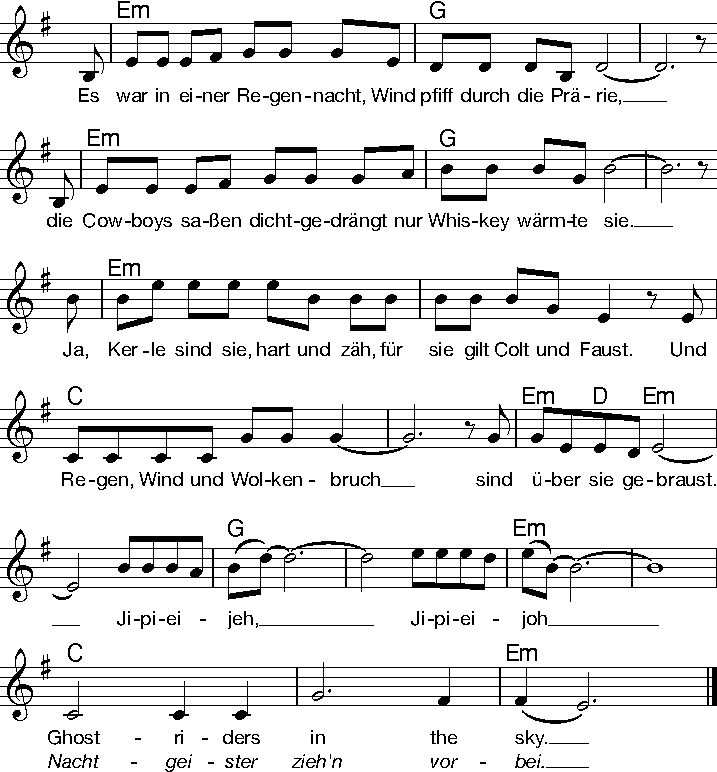
\includegraphics[width=1\textwidth]{Noten/Lied041.pdf}	

\beginverse
Da \[Em]tritt der Teufel in den Kreis und \[G]winkt dem einen zu;
der \[Em]wendet sich verzweifelt um, beim \[G]Himmel sucht er Ruh'.
\[Em]Zu den Sternen will er flüchten, zur Sonne will er flieh'n,
doch \[C]alle Sterne werden bleich und die \[Em]Sonne \[D]will ver\[Em]glüh'n.
\endverse

\beginchorus
Ji-pi-ei-\[G]jeh - ji-pi-ei-\[Em]joh, \[C]ghostriders in the \[Em]sky.
\endchorus

\beginverse
Da ^öffnet sich der Himmel weit und ^Reiter kommen aus Höh'n
und ^Feuer sprüht aus Pferdenüstern, ^wilde Winde weh'n.
Der ^tote Cowboy wird genommen und keiner wird gefragt
und ^weiter geht es aufwärts in ^wilder, ^toller ^Jagd.
\endverse

\beginchorus
\lrep Ji-pi-ei-\[G]jeh - ji-pi-ei-\[Em]joh, \[C]ghostriders in the \[Em]sky. \rrep
\endchorus

\endsong

\beginscripture{}
Das Lied heißt im Englischen original ''Ghostriders in the Sky'' und wurde durch ein Cover Johnny Cashs bekannt.
\endscripture
